\section{Computer vision using neural networks}
It was required that the system detect the position of an object from a photo. In particular, the object detector should,

\begin{itemize}
	\item not require a beacon or light to be placed on the object,
	\item run at around 5 to 10 Hz,
	\item locate the object with high accuracy,
	\item work regardless of the orientation of the object, and
	\item be able to track any object with minimal extra work/design required.
\end{itemize}

This chapter details the literature sounding methods which could potentially achieve these requirements.

\subsection{Basic computer vision concepts}
Computer vision techniques tend to use a number of cascaded filters, with each layer of filters being able to detect more and more complex shapes in an image. These filters are known as 'kernels', and tend to be implemented as \pyth{3x3} matrices which are convolved with the input image, a 2D array of pixel values.

As an example, plotted below is an image before (left) and after (right) being convolved with a vertical line finding kernel.

\begin{figure}[h!]%
    \centering
    \subfloat{{
\includegraphics[width=3cm]{literature_review/input_image} }}%
    \qquad \qquad
    \subfloat{{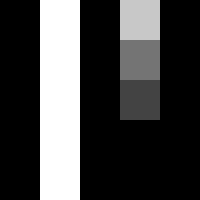
\includegraphics[width=3cm]{literature_review/output_image} }}%
    \caption{An image, before (left) and after (right) being convolved with a vertical line finder.}%
    \label{fig:example}%
\end{figure}

Note how the the vertical line in left part of the input has been found (represented by bright pixels in the output image). The horizontal line on the bottom right has been rejected. The faint vertical line in the top right has been found, albeit faintly. The exact same transformation is shown below, where the leftmost matrix is the input, the middle is the kernel and the rightmost matrix is the output.

\begin{table}[h!]
	\centering
	\begin{tabular}{ p{0.5cm} p{0.5cm} p{0.5cm} p{0.5cm} p{0.5cm} p{0.5cm} p{0.5cm} p{0.5cm} p{0.5cm} p{0.5cm} p{0.5cm} p{0.5cm} p{0.5cm} p{0.5cm} p{0.5cm}}
		 5 & 232 & 180 & 212 & 180 &           &    &   &    &   & 0 & 255 & 0 & 200 & 0 \\
		30 & 243 & 152 & 206 & 188 &           & -1 & 2 & -1 &   & 0 & 255 & 0 & 116 & 0 \\
		32 & 255 & 210 & 190 & 190 & $\otimes$ & -1 & 2 & -1 & = & 0 & 255 & 67 & 0  & 0 \\
		11 & 242 & 235 & 230 & 210 &           & -1 & 2 & -1 &   & 0 & 255 & 0 &  0  & 0 \\
		90 & 240 & 130 &  20 &  30 &           &    &   &    &   & 0 & 255 & 0 &  0  & 0
	\end{tabular}
\end{table}

A larger, more interesting input image is shown below, in Figure~\ref{fig:image_kernel_demo}.

\begin{figure}[h!]
  \centering
  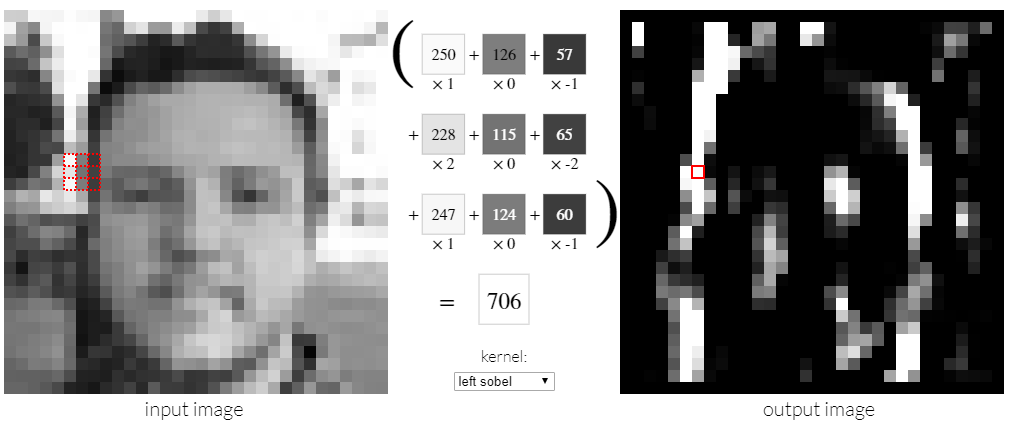
\includegraphics[width=\textwidth]{literature_review/image_kernel_demo}
  \caption{\label{fig:image_kernel_demo} A demonstration of image convolution on a photo of a human.}
\end{figure}

As an example of a complete system, the first layer of kernels may detect vertical lines, angled lines, dots, and so on. These detections are then used as input matrices to the next layer, which will convolve them with a set of kernels to produce more complex detections. For example, two horizontal lines and two vertical lines may indicate the presence of a square in an image. A different configuration of lines may indicate a circle, and so on.

Carefully designing and combining these filters can ultimately result in the detection of an object. However, this method is incredibly time consuming and requires extensive domain-specific knowledge. Even after the work has been put in to locate one type of object in a frame, locating another type of object may require the user to start from scratch.

\subsection{Introduction to machine learning}

Luckily, there exist other methods of creating and combining the kernels mentioned previously. Instead of hand-crafting each kernel and deciding how they should be combined, one could instead use machine-learning techniques (in which a computer can use a dataset of input-output pairs to learn the parameters of a model) to create kernels with 'optimal' values to find objects in a frame. This boils down to using data (known input-output pairs of an image of cheetah, and the label "cheetah") to optimize neural network.

The standard method of doing this for images is through the use of Convolutional Neural Networks (CNNs). CCNs are initialized with random values in their kernels and random weights which combine the outputs of their kernels - only their general architecture is fixed by human practitioners. The method to get accurate weights is then as follows:

\begin{enumerate}
\item Initialize the CNN with random values in the kernels and weights between 'neurons' (nodes in the CNN which perform an operation).
\item Pass an image through all the neurons in the CNN, and take note of the output.
\item Get the error (the difference between the CNN output and the correct answer) and propagate it back through the CNN, adjusting the weights \emph{slightly} in such a way that that same input would produce the correct output if run again.
\item Repeat the first three steps a few hundred or thousand times, using a large, diverse dataset.
\end{enumerate}

While it is possible that the CNN will act as a look-up table (mapping those specific inputs to their correct outputs, but giving the wrong result for any other dataset) it is hoped that the CNN will instead map any \emph{similar} input to the correct output. As an example, a correct training CNN will map any image which \emph{looks} like a cheetah (has the correct body structure, spots, ear location, etc) to an output which is numerically encoded to represent "cheetah".

It should be noted that CNNs are nothing more than a mapping from a vector of input pixels to a vector which represents certain outputs (such as "cheetah", "no cheetah" or even the coordinates of a cheetah).

CNNs simply require a few hundred or thousand labelled images and a few hours on a modern GPU. There are many open datasets which can be used to make this work easier.

\subsection{Key machine learning concepts and definitions}
Before getting lost in ReLU, dropout and the rest of the endless list of ideas in machine learning, it is worth considering the separation of jobs in in modern data science. Typically, there is one team which designs the neural network architecture, tunes hyper-parameters (import parameters usually set by humans), publishes results, and son on. This requires a certain set of skills.

Next, another person with a separate skill set puts the neural network in production in order to achieve some goal, possibly after training it them self. If you find yourself in the second group of people, you don't tend to need to keep up with every new paper published. Instead, armed with some understanding of the main innovations in each network design, you only need compare training techniques and architectures as a whole.

Since the project at hand doesn't necessitate a brand new architecture, only a handful ideas need to be discussed.

\textit{Machine learning, neural networks, deep learning, CNNs}: machine learning is the branch of computer science involved in fitting a model using data alone. Neural networks are a subset of machine learning, specifying a class of architectures loosely inspired by the synapses in the nervous system of an organic brain. Deep learning is the relatively recent practice of creating especially long neural networks in order to represent more complex mappings. Finally, CNNs are a subset of deep learning, in which the synapses of a deep neural network are kernels which perform convolution operations.

\textit{Image classification vs object detection:} an image classifier indicates \emph{what} object(s) are in an image. An object detector finds what objects are in the image, and also \emph{where} in the image they can be found.

\textit{Bounding box: (or 'anchor'):} a pair of points which determine a box around a detected object.

\textit{Feature extractor:} it is common practice to concatenate an well-designed existing neural network with another architecture to produce a new, larger model which performs an overall more complex task. Thus, the role of the first part of the new model is to extract useful features for the second part to process.

\textit{Transfer learning:} this refers to the practice in which the weights of one neural network are copied to another network. This enables problems to be solved using much less data than neural networks ordinarily require, as the weights are already quite good before the retraining process. The idea is that the early layers are likely to have been trained to find very general features in the image (such as lines, circles, eyes, tails, etc). These are often relevant to a wide variety of problems. This is why a trained network will often have its training dataset specified - the content of the training dataset is a good indicator of whether transfer learning would help in a different problem.

\textit{Epoch:}

\textit{Batch size:}

\textit{Loss:}

\subsection{Movidius Neural Compute stick}
CNNs tend to require a large number of operations to produce an output. The exact amount of computation required depends on the neural network architecture, though even 'small' object detectors generally require on the order of millions of multiply-accumulate instructions with significant amounts of data being loaded to and from the various levels of cache. Combined with the slower processor on embedded computers such as a raspberry pi, the neural network would not be able to run in real time (inference time less than $\approx 100ms$). As an example, a cutting edge object detection network designed for use on mobile devices requires about 1 second to infer a result on the raspberry pi's CPU.

% nn and params: https://mxnet.apache.org/api/python/gluon/model_zoo.html

Fortunately, this work can be easily parallelised over multiple processing cores. There are three types of parallelization which tend to occur - during the application of kernels, during matrix multiplication and in parts of the neural network where the data flow is naturally parallel. This work is a perfect fit for GPUs, which contain a large number of processing cores designed for such tasks. However, since GPU support for CNNs on the raspberry pi is lacking, other means had to be investigated.

% https://petewarden.com/2014/08/07/how-to-optimize-raspberry-pi-code-using-its-gpu/
% https://rpiplayground.wordpress.com/2014/05/03/hacking-the-gpu-for-fun-and-profit-pt-1/

\textit{For the rest of this chapter, assume any obscure words have been patented by Intel$^{^{\ TM}}$ or one of its subsidiaries.}

To solve this problem, some chip makers have started to produce 'neural accelerators' - devices which can be used to decrease the inference time of neural network. One such as the Movidius Neural Compute Stick (NCS) - a specialized neural network accelerator which plugs into the raspberry pi (or any other computer). Its 12 purpose-built processing cores typically result in inference speed increases of between $700\%$ and $1000\%$. It also has the benefit of being purpose built for CNNs.

The operation of the Movidius NCS is as follows: first, the user designs and trains their neural network. Next, they compile it down to a device-specific format optimized for the NCS and upload it to the device. From then on, the user can send preprocessed images to the devices, wait for the inference to occur, and then retrieve the result.

The actual processing is done using Intel's Myriad 2 Vision Processing Unit (VPU), which makes use of 12 specially designed processing cores named 'shaves'.

%\begin{figure}[h!]
%  \centering
%  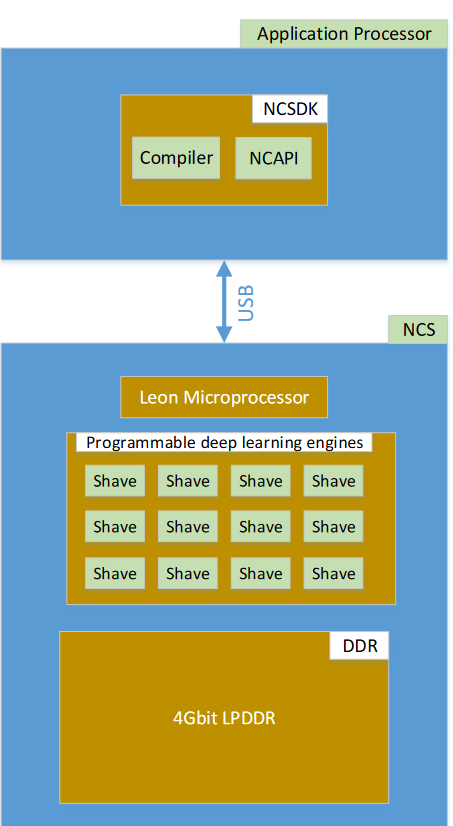
\includegraphics[width=0.4\textwidth]{literature_review/NCS_internals}
%  \caption{\label{fig:NCS_internals} Internals of the Movidius Neural Compute Stick.}
%\end{figure}



\subsection{Comparison of neural network architectures}
Not all neural network architectures are equal - generally, differences between models include,

\begin{itemize}
	\item Classification accuracy,
	\item Inference speed, which is a function of
	\begin{itemize}
		\item The number of operations (processing) and
		\item The number of weights (data retrieval)
	\end{itemize}
	\item The amount of data required for training/fine tuning,
	\item The existence (or lack) of pretrained models in each specific deep learning framework,
	\item Whether recent innovations in the field have been included, and
	\item The underlying method in which objects are detected and localised within the image
\end{itemize}


Newer neural networks often take ideas from older architectures. Sometimes, they even include all or most of a previous architecture as part of the design of the new model. An example of this is MobileNet - an architecture designed at Google, aimed to run quickly on modern mobile devices (such as their newer smartphones). A common practice is to train MobileNet to classify objects on a given dataset, then remove the final layers, concatenate it with another model (with MobileNet acting as a feature extractor) and end up with an object detector.

Since MobileNet was designed for mobile devices, it traded some classification accuracy for performance. However, the architecture is remarkable in that the performance increase is significant while the classification accuracy decrease is not. Thus, it was chosen as the feature detector for the project.

Next was the choice of the actual object detector. There are two (TODO: check this) main ideas for this approach: one could get an image classifier and apply it to the image multiple times (such as 25 times) resulting in a grid of overlapping detections.

{\Large Show image here}
\hrule

Using the prediction probability for each part of the image, one can estimate where in the frame the desire object(s) is. This has the advantage of allowing for a simpler network architecture, but comes at the cost of performance (as the neural network must be applied multiple times) and resolution (determined by the grid size, which determines the run time). This is known as the 'sliding window' technique.

The other approach uses the fact that the neural network can locate objects in the frame, and thus returns the locations of objects in the image embedded in the output nodes. An example of this type of network is the Single Shot Detector (SSD) which, as the name suggests, requires only a single inference to output a list of objects, their classification probabilities and their locations in the frame.

[ TODO: RESULTS: talk about trying to make my own network with two output nodes, which simply predicts the centroid of the object as a scale from -1 to 1, with -1 being the bottom or left side of the image and 0 being the center. Couldn't get it to compile due to tensorflow support ]

\subsection{Comparison of neural network frameworks}
% speeds: https://arxiv.org/pdf/1608.07249v7.pdf
Tensorflow - low level, annoying and hard to use, fast
Keras - simple to use, tensorflow as backend so relatively fast, less fine grained control possible, can't find all the latest models there, can export model as tensorflow
Caffe - fast, easy to use, hard to extend, only really for CNNs, might be dying out
